\chapter{GNU Makefiles}

\includegraphics[scale=0.20]{images/books-1163695_1920.jpg}

\justify{}
The GNU make tool is a handy way to put short sets of oft-repeated steps at the fingertips of the
developer. For make to function properly, you must create a Makefile\index{Makefile} in the directory
you invoke the make command from. Using a Makefile lets us avoid typing complicated and hard to recall strings on the command
line. You can simply type ``make docker'' and have everything build as desired. This is beneficial when
you have lots of arguments and environment variables that you and your team members need for sets of commands
to work properly. When your team member invokes a specific rule from a Makefile, it works without you having to 
help them configure things or make them aware of all the parameters.
We're going to be using \href{https://www.gnu.org/software/make/}{GNU Make} for our projects.

\section{Anatomy of a Makefile}

\justify{}
A Makefile can be as simple as a few lines or grow to become an extremely intricate and vital piece of your
build environment. You might like to have a look at 
\href{https://www.gnu.org/software/make/manual/make.html#Introduction}{the GNU make manual} at least once just to get a feel for how they work.

\justify{}
When a Makefile is executed, you can use the ampersand character to suppress the printing of lines from the original Makefile.

\section{Rules}

\justify{}
Makefiles are comprised of various stanzas, know as rules. This is where the work gets done. Let's add a rule
for Docker and a target for Python to make our lives easier in the future. Let's examine a simple Makefile with a single rules.

\justify{}
\begin{mybox}{\thetcbcounter: Our First Makefile}
	\lstinputlisting{code/23-makefiles/simple-makefile}
\end{mybox}

\justify{}
It's important to note that indentation of Makefiles is done using tabs rather than spaces. If your Makefile is failing, check for spots where lines were improperly indented with eight spaces. The proper way to indent in a Makefile is to use tab characters.

\section{The PHONY Directive}

\justify{}
If a file or directory exists with the same name as a rule in the Makefile, you will need to specify
it under the \emph{PHONY} directive. This will allow the Makefile to find and run the desired commands.

\justify{}
\begin{mybox}{\thetcbcounter: The PHONY Directive}
	\lstinputlisting{code/23-makefiles/phony-makefile}
\end{mybox}

\markdownInput{../labs/ch6/lab-6a.md}
	
\section{Rules}

\justify{}
Makefiles are comprised of various stanzas, know as rules. This is where the work gets done. Let's add a rule
for Docker and a target for Python to make our lives easier in the future. Consider the two rules below.

\justify{}
\begin{mybox}{\thetcbcounter: A Makefile Target}
	\lstinputlisting{code/23-makefiles/makefile-target}
\end{mybox}

\justify{}
When the user types ``make docker'' at the CLI to invoke the docker target in the Makefile, the fist thing
that happens is the python rule is called. If the file python/requirements.txt exists, we attempt to install
the modules listed within that requirements file using the Python ``pip'' package manager. Once completed, the
thread of execution returns to the docker target. A message is sent to the user via STDOUT
that we will be building with docker-compose. An empty file at the root of the containers filesystem named /.dockerenv
is a convention that indicates we are operating inside a containerized environment. After a quick check for
existence of the file /.dockerenv, we use docker-compose to build from our Dockerfile, and then start a BASH shell in our ``cloudlab'' container. The user now has the ability to run BASH commands
``inside'' the Docker container.

\justify{}
Be sure when you indent in a Makefile that you use tabs, not spaces. You can use the backslash character in a Makefile to combine two consecutive
lines into one logical line.

\section{A Simple Makefile Exmaple}

\justify{}
Let's look at a simple Makefile example. 

\section{Full Example Makefile}
\justify{}
Next, let's look at a full working example of a Makefile.

\section{Directory Structure with Makefile}
\justify{}
Relevant files and folders related to our Makefile are organized as seen
below.

\begin{figure}[!htb]
	
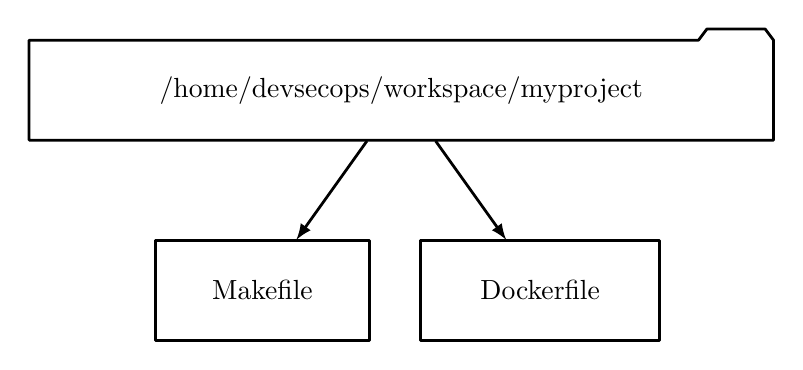
\begin{tikzpicture}[>=latex,line join=bevel,]
  \pgfsetlinewidth{1bp}
%%
\pgfsetcolor{black}
  % Edge: devsecops -> Makefile
  \draw [->] (121.64bp,71.697bp) .. controls (115.77bp,63.474bp) and (108.63bp,53.483bp)  .. (96.217bp,36.104bp);
  % Edge: devsecops -> Dockerfile
  \draw [->] (146.36bp,71.697bp) .. controls (152.23bp,63.474bp) and (159.37bp,53.483bp)  .. (171.78bp,36.104bp);
  % Node: devsecops
\begin{scope}
  \definecolor{strokecol}{rgb}{0.0,0.0,0.0};
  \pgfsetstrokecolor{strokecol}
  \draw (268.0bp,108.0bp) -- (265.0bp,112.0bp) -- (244.0bp,112.0bp) -- (241.0bp,108.0bp) -- (0.0bp,108.0bp) -- (0.0bp,72.0bp) -- (268.0bp,72.0bp) -- cycle;
  \draw (134.0bp,90.0bp) node {/home/devsecops/workspace/myproject};
\end{scope}
  % Node: Makefile
\begin{scope}
  \definecolor{strokecol}{rgb}{0.0,0.0,0.0};
  \pgfsetstrokecolor{strokecol}
  \draw (122.5bp,36.0bp) -- (45.5bp,36.0bp) -- (45.5bp,0.0bp) -- (122.5bp,0.0bp) -- cycle;
  \draw (84.0bp,18.0bp) node {Makefile};
\end{scope}
  % Node: Dockerfile
\begin{scope}
  \definecolor{strokecol}{rgb}{0.0,0.0,0.0};
  \pgfsetstrokecolor{strokecol}
  \draw (227.0bp,36.0bp) -- (141.0bp,36.0bp) -- (141.0bp,0.0bp) -- (227.0bp,0.0bp) -- cycle;
  \draw (184.0bp,18.0bp) node {Dockerfile};
\end{scope}
%
\end{tikzpicture}


	\caption{Makefile and related files.}
\label{makefile}
\end{figure}

